% Created 2019-06-19 三 14:49
% Intended LaTeX compiler: pdflatex
\documentclass[11pt]{article}
\usepackage[utf8]{inputenc}
\usepackage[T1]{fontenc}
\usepackage{graphicx}
\usepackage{grffile}
\usepackage{longtable}
\usepackage{wrapfig}
\usepackage{rotating}
\usepackage[normalem]{ulem}
\usepackage{amsmath}
\usepackage{textcomp}
\usepackage{amssymb}
\usepackage{capt-of}
\usepackage{hyperref}
\usepackage{minted}
\graphicspath{{../../images/ArtificialIntelligence/}}
% TIPS
% \substack{a\\b} for multiple lines text





% pdfplots will load xolor automatically without option
\usepackage[dvipsnames]{xcolor}

\usepackage{forest}
% two-line text in node by [two \\ lines]
% \begin{forest} qtree, [..] \end{forest}
\forestset{
  qtree/.style={
    baseline,
    for tree={
      parent anchor=south,
      child anchor=north,
      align=center,
      inner sep=1pt,
    }}}
%\usepackage{flexisym}
% load order of mathtools and mathabx, otherwise conflict overbrace

\usepackage{mathtools}
%\usepackage{fourier}
\usepackage{pgfplots}
\usepackage{amsthm}
\usepackage{amsmath}
%\usepackage{unicode-math}
%
\usepackage{commath}
%\usepackage{,  , }
\usepackage{amsfonts}
\usepackage{amssymb}
% importing symbols https://tex.stackexchange.com/questions/14386/importing-a-single-symbol-from-a-different-font
%mathabx change every symbol
% use instead stmaryrd
%\usepackage{mathabx}
\usepackage{stmaryrd}
\usepackage{empheq}
\usepackage{tikz}
\usepackage{tikz-cd}
%\usepackage[notextcomp]{stix}
\usetikzlibrary{arrows.meta}
\usepackage[most]{tcolorbox}
%\utilde
%\usepackage{../../latexpackage/undertilde/undertilde}
% left and right superscript and subscript
\usepackage{actuarialsymbol}
\usepackage{threeparttable}
\usepackage{scalerel,stackengine}
\usepackage{stackrel}
% \stackrel[a]{b}{c}
\usepackage{dsfont}
% text font
\usepackage{newpxtext}
%\usepackage{newpxmath}

%\newcounter{dummy} \numberwithin{dummy}{section}
\newtheorem{dummy}{dummy}[section]
\theoremstyle{definition}
\newtheorem{definition}[dummy]{Definition}
\newtheorem{corollary}[dummy]{Corollary}
\newtheorem{lemma}[dummy]{Lemma}
\newtheorem{proposition}[dummy]{Proposition}
\newtheorem{theorem}[dummy]{Theorem}
\theoremstyle{definition}
\newtheorem{example}[dummy]{Example}
\theoremstyle{remark}
\newtheorem*{remark}{Remark}


\newcommand\what[1]{\ThisStyle{%
    \setbox0=\hbox{$\SavedStyle#1$}%
    \stackengine{-1.0\ht0+.5pt}{$\SavedStyle#1$}{%
      \stretchto{\scaleto{\SavedStyle\mkern.15mu\char'136}{2.6\wd0}}{1.4\ht0}%
    }{O}{c}{F}{T}{S}%
  }
}

\newcommand\wtilde[1]{\ThisStyle{%
    \setbox0=\hbox{$\SavedStyle#1$}%
    \stackengine{-.1\LMpt}{$\SavedStyle#1$}{%
      \stretchto{\scaleto{\SavedStyle\mkern.2mu\AC}{.5150\wd0}}{.6\ht0}%
    }{O}{c}{F}{T}{S}%
  }
}

\newcommand\wbar[1]{\ThisStyle{%
    \setbox0=\hbox{$\SavedStyle#1$}%
    \stackengine{.5pt+\LMpt}{$\SavedStyle#1$}{%
      \rule{\wd0}{\dimexpr.3\LMpt+.3pt}%
    }{O}{c}{F}{T}{S}%
  }
}

\newcommand{\bl}[1] {\boldsymbol{#1}}
\newcommand{\Wt}[1] {\stackrel{\sim}{\smash{#1}\rule{0pt}{1.1ex}}}
\newcommand{\wt}[1] {\widetilde{#1}}
\newcommand{\tf}[1] {\textbf{#1}}


%For boxed texts in align, use Aboxed{}
%otherwise use boxed{}

\DeclareMathSymbol{\widehatsym}{\mathord}{largesymbols}{"62}
\newcommand\lowerwidehatsym{%
  \text{\smash{\raisebox{-1.3ex}{%
    $\widehatsym$}}}}
\newcommand\fixwidehat[1]{%
  \mathchoice
    {\accentset{\displaystyle\lowerwidehatsym}{#1}}
    {\accentset{\textstyle\lowerwidehatsym}{#1}}
    {\accentset{\scriptstyle\lowerwidehatsym}{#1}}
    {\accentset{\scriptscriptstyle\lowerwidehatsym}{#1}}
}

\usepackage{graphicx}
    
% text on arrow for xRightarrow
\makeatletter
%\newcommand{\xRightarrow}[2][]{\ext@arrow 0359\Rightarrowfill@{#1}{#2}}
\makeatother


\newcommand{\dom}[1]{%
\mathrm{dom}{(#1)}
}

% Roman numerals
\makeatletter
\newcommand*{\rom}[1]{\expandafter\@slowromancap\romannumeral #1@}
\makeatother

\def \fR {\mathfrak{R}}
\def \bx {\boldsymbol{x}}
\def \bz {\boldsymbol{z}}
\def \ba {\boldsymbol{a}}
\def \bh {\boldsymbol{h}}
\def \bo {\boldsymbol{o}}
\def \bU {\boldsymbol{U}}
\def \bc {\boldsymbol{c}}
\def \bV {\boldsymbol{V}}
\def \bI {\boldsymbol{I}}
\def \bK {\boldsymbol{K}}
\def \bt {\boldsymbol{t}}
\def \bb {\boldsymbol{b}}
\def \bA {\boldsymbol{A}}
\def \bX {\boldsymbol{X}}
\def \bu {\boldsymbol{u}}
\def \bS {\boldsymbol{S}}
\def \bZ {\boldsymbol{Z}}
\def \bz {\boldsymbol{z}}
\def \by {\boldsymbol{y}}
\def \bw {\boldsymbol{w}}
\def \bT {\boldsymbol{T}}
\def \bF {\boldsymbol{F}}
\def \bS {\boldsymbol{S}}
\def \bm {\boldsymbol{m}}
\def \bW {\boldsymbol{W}}
\def \bR {\boldsymbol{R}}
\def \bQ {\boldsymbol{Q}}
\def \bS {\boldsymbol{S}}
\def \bP {\boldsymbol{P}}
\def \bT {\boldsymbol{T}}
\def \bY {\boldsymbol{Y}}
\def \bH {\boldsymbol{H}}
\def \bB {\boldsymbol{B}}
\def \blambda {\boldsymbol{\lambda}}
\def \bPhi {\boldsymbol{\Phi}}
\def \btheta {\boldsymbol{\theta}}
\def \bTheta {\boldsymbol{\Theta}}
\def \bmu {\boldsymbol{\mu}}
\def \bphi {\boldsymbol{\phi}}
\def \bSigma {\boldsymbol{\Sigma}}
\def \lb {\left\{}
\def \rb {\right\}}
\def \la {\langle}
\def \ra {\rangle}
\def \caln {\mathcal{N}}
\def \dissum {\displaystyle\Sigma}
\def \dispro {\displaystyle\prod}
\def \E {\mathbb{E}}
\def \Q {\mathbb{Q}}
\def \N {\mathbb{N}}
\def \V {\mathbb{V}}
\def \R {\mathbb{R}}
\def \P {\mathbb{P}}
\def \A {\mathbb{A}}
\def \Z {\mathbb{Z}}
\def \I {\mathbb{I}}
\def \C {\mathbb{C}}
\def \cala {\mathcal{A}}
\def \calb {\mathcal{B}}
\def \calq {\mathcal{Q}}
\def \calp {\mathcal{P}}
\def \cals {\mathcal{S}}
\def \calg {\mathcal{G}}
\def \caln {\mathcal{N}}
\def \calr {\mathcal{R}}
\def \calm {\mathcal{M}}
\def \calc {\mathcal{C}}
\def \calf {\mathcal{F}}
\def \calk {\mathcal{K}}
\def \call {\mathcal{L}}
\def \calu {\mathcal{U}}
\def \bcup {\bigcup}


\def \uin {\underline{\in}}
\def \oin {\overline{\in}}
\def \uR {\underline{R}}
\def \oR {\overline{R}}
\def \uP {\underline{P}}
\def \oP {\overline{P}}

\def \Ra {\Rightarrow}

\def \e {\enspace}

\def \sgn {\operatorname{sgn}}
\def \gen {\operatorname{gen}}
\def \ker {\operatorname{ker}}
\def \im {\operatorname{im}}

\def \tril {\triangleleft}

% \varprod
\DeclareSymbolFont{largesymbolsA}{U}{txexa}{m}{n}
\DeclareMathSymbol{\varprod}{\mathop}{largesymbolsA}{16}

% \bigtimes
\DeclareFontFamily{U}{mathx}{\hyphenchar\font45}
\DeclareFontShape{U}{mathx}{m}{n}{
      <5> <6> <7> <8> <9> <10>
      <10.95> <12> <14.4> <17.28> <20.74> <24.88>
      mathx10
      }{}
\DeclareSymbolFont{mathx}{U}{mathx}{m}{n}
\DeclareMathSymbol{\bigtimes}{1}{mathx}{"91}
% \odiv
\DeclareFontFamily{U}{matha}{\hyphenchar\font45}
\DeclareFontShape{U}{matha}{m}{n}{
      <5> <6> <7> <8> <9> <10> gen * matha
      <10.95> matha10 <12> <14.4> <17.28> <20.74> <24.88> matha12
      }{}
\DeclareSymbolFont{matha}{U}{matha}{m}{n}
\DeclareMathSymbol{\odiv}         {2}{matha}{"63}


\newcommand\subsetsim{\mathrel{%
  \ooalign{\raise0.2ex\hbox{\scalebox{0.9}{$\subset$}}\cr\hidewidth\raise-0.85ex\hbox{\scalebox{0.9}{$\sim$}}\hidewidth\cr}}}
\newcommand\simsubset{\mathrel{%
  \ooalign{\raise-0.2ex\hbox{\scalebox{0.9}{$\subset$}}\cr\hidewidth\raise0.75ex\hbox{\scalebox{0.9}{$\sim$}}\hidewidth\cr}}}

\newcommand\simsubsetsim{\mathrel{%
  \ooalign{\raise0ex\hbox{\scalebox{0.8}{$\subset$}}\cr\hidewidth\raise1ex\hbox{\scalebox{0.75}{$\sim$}}\hidewidth\cr\raise-0.95ex\hbox{\scalebox{0.8}{$\sim$}}\cr\hidewidth}}}
\newcommand{\stcomp}[1]{{#1}^{\mathsf{c}}}


\author{wu}
\date{\today}
\title{Artificial Intelligence}
\hypersetup{
 pdfauthor={wu},
 pdftitle={Artificial Intelligence},
 pdfkeywords={},
 pdfsubject={},
 pdfcreator={Emacs 26.2 (Org mode 9.2.4)}, 
 pdflang={English}}
\begin{document}

\maketitle
\tableofcontents

\section{Inference and Reasoning}
\label{sec:org19afaa7}
\subsection{Propositional logic}
\label{sec:org6c9898a}
\subsection{Predicate logic}
\label{sec:org36736b4}
\subsection{First Order Inductive Learner}
\label{sec:org972d501}
\textbf{knowledge graph}: node = entity, edge = relation.
triplet (head entity, relation, tail entity)
\section{Statistical learning and modeling}
\label{sec:orgf111181}
\subsection{Machine Learning: the concept}
\label{sec:org09afdc3}
\subsubsection{Example and concept}
\label{sec:orgcfcfc9c}
\begin{description}
\item[{Supervised learning problems}] applications in which the \textbf{training data} comprises examples of the input
vectors along with their corresponding \textbf{target vectors} are known

classification and regression
\item[{Unsupervised learning problems}] the training data consists of a set of input vectors X \textbf{without any
corresponding target values}

density estimation, clustering, hidden markov models
\item[{Reinforcement learning problem}] finding suitable actions to take in a given situation in order to
maximize a reward. Here the learning algorithm is not given examples of
optimal outputs, in contrast to supervised learning, but must instead
discover them by a process of trial and error. A general feature of
reinforcement learning is the trade-off between exploration and exploitation
\end{description}

types of machine learning
\begin{itemize}
\item supervised learning
\begin{itemize}
\item classification: the output is categorical or nominal variable
\item regression: the output is read-valued variable
\end{itemize}
\item unsupervised learning
\item semi-supervised learning
\item reinforcement learning
\item deep learning
\end{itemize}
\subsubsection{supervised learning: important concepts}
\label{sec:orgd148b47}
\begin{itemize}
\item Data: labeled instances \(<\bl{x}_i,\bl{y}>\)
\item features: attribute-value pairs which characterize each \(\bl{x}\)
\item learning a discrete function: \textbf{classification}
\item learning a continuous function: \textbf{regression}
\end{itemize}

\textbf{Classification} - A two-step process
\begin{itemize}
\item \textbf{model construction}
\item \textbf{model usage}
\end{itemize}

\textbf{regression}
\begin{itemize}
\item Example: price of a used car

\(\bl{x}\): car attributes. \(\bl{y}=g(\bl{x}\mid\bl{\theta})\): price. \(g\):
model. \(\theta\) parameter set.
\end{itemize}
\subsection{example: polynomial curve fitting}
\label{sec:orgc129115}
\subsection{probability theory review and notation}
\label{sec:org859dde0}
rules of probability
\begin{itemize}
\item \textbf{sum rule} \(p(X)=\displaystyle\sum_Yp(X,Y)\)
\item \textbf{product rule} \(p(X,Y)=p(Y|X)p(X)\)
\end{itemize}

Bayes' Theorem: \(p(Y|X)=\frac{p(X|Y)p(Y)}{p(X)}\). Using sum rule
\(p(X)=\displaystyle\sum_Yp(X|Y)p(Y)\)

probability densities. 
\begin{align*}
p(x\in(a,b))&=\int_a^bp(x)dx\\
P(z)&=\int_{-\infty}^z p(x)dx\\
\int_{-\infty}^\infty p(x)dx&=1\quad p(x)\le0
\end{align*}


\textbf{expectation} \(\mathbb{E}[f]=
   \begin{cases}
   \displaystyle\sum_{x}p(x)f(x) & \text{discrete variables}\\
   \int p(x)f(x)dx & \text{continuous variables}
   \end{cases}\). In either cases,
\(\mathbb{E}[f]\approx\frac{1}{N}\displaystyle\sum_{n=1}^N f(x_n)\).
\textbf{conditional expectation}: \(\mathbb{E}_x[f| y]=\displaystyle\sum_xp(x| y)f(x)\).

The \textbf{variance} of \(f(x)\) is

\begin{align*}
var[f]&=\mathbb{E}[(f(x)-\mathbb{E}[f(x)])^2]\\
&=\mathbb{E}[f(x)^2-2f(x)\mathbb{E}[f(x)]+\mathbb{E}[f(x)]^2]\\
&=\mathbb{E}[f(x)^2]-\mathbb{E}[f(x)]^2
\end{align*}


The \textbf{covariance} is

\begin{align*}
cov[x,y]&=\mathbb{E}_{x,y}[(x-\mathbb{E}[x])(y-\mathbb{E}[y])]\\
&=\mathbb{E}_{x,y}[xy]-\mathbb{E}[x]\mathbb{E}[y]
\end{align*}


\emph{the variance of the sum of two independent random variables is the sum of}
\emph{variance}. Given
\begin{center}
\begin{tabular}{c|c}
X & probability\\
\hline
\(x_1\) & \(p_1\)\\
\(\dots\) & \(\dots\)\\
\(x_n\) & \(p_n\)\\
\end{tabular}
\end{center}

\begin{center}
\begin{tabular}{c|c}
Y & probability\\
\hline
\(y_1\) & \(q_1\)\\
\(\dots\) & \(\dots\)\\
\(y_m\) & \(q_m\)\\
\end{tabular}
\end{center}
\begin{align*}
var(X+Y)=var(X)+var(Y)
\end{align*}

In case of two vectors of random variables \(\bl{x}\) and \(\bl{y}\), the
covariance is a matrix
\begin{align*}
cov[\bl{x},\bl{y}]&=\mathbb{E}_{\bl{x},\bl{y}}[(\bl{x}-\mathbb{E}[\bl{x}])(\bl{y}^T
-\mathbb{E}[\bl{y}^T])]\\
&=\mathbb{E}_{\bl{x},\bl{y}}[\bl{xy}^T]-\mathbb{E}[\bl{x}]\mathbb{E}[\bl{y}^T]
\end{align*}

\textbf{Bayesian probabilities}: \(P(A|B)=\frac{P(B|A)P(A)}{P(B)}\). For a data set 
\(\mathcal{D}=\{t_1,\dots,t_n\}\) and assumption \(w\),
\(p(w|\mathcal{D})=\frac{p(\mathcal{D}|w)p(w)}{p(\mathcal{D})}\). \(p(w)\) is
\textbf{prior probability}, \(p(\mathcal{D}|w)\) is \textbf{likelihood} (the probability
\(\mathcal{D}\) happens). Hence 
\begin{equation*}
\text{posterior}\propto\text{likelihood}\times\text{prior}
\end{equation*}

\textbf{Gaussian distribution}.
\begin{equation*}
\mathcal{N}(x|\mu,\sigma^2)=\frac{1}{(2\pi\sigma^2)^{1/2}}\exp\left\{
-\frac{1}{2\sigma^2}(x-\mu)^2\right\}
\end{equation*}
\(\mu\) is called \textbf{mean}, \(\sigma^2\) is called \textbf{variance}, \(\sigma\) \textbf{standard
deviation}, \(\beta=1/\sigma^2\) \textbf{precision}
\begin{align*}
\mathbb{E}[x]&=\int_{-\infty}^\infty\mathcal{N}(x|\mu,\sigma^2)xdx=\mu\\
\mathbb{E}[x^2]&=\int_{-\infty}^\infty\mathcal{N}(x|\mu,\sigma^2)x^2dx=\mu^2
+\sigma^2\\
var[x]&=\mathbb{E}[x^2]-\mathbb{E}[x]^2=\sigma^2\\
\end{align*}
For \$D\$-dimensional vector \(\bl{x}\) of continuous variables
\begin{equation*}
\mathcal{N}(\bl{x}|\bl{\mu},\bl{\Sigma})=\frac{1}{(2\pi)^{D/2}}\frac{1}
{\abs{\bl{\Sigma}}^{1/2}}\exp\left\{-\frac{1}{2}(\bl{x}-\bl{\mu})^T
\bl{\Sigma^{-1}}(\bl{x}-\bl{\mu})\right\}
\end{equation*}

To determine values for the unknown parameters given \(\mu\) and \(\sigma^2\) by
maximizing the likelihood function. Use log.
\begin{align*}
P(\bl{X}|\mu,\sigma^2)&=\displaystyle\prod_{n=1}^N\mathcal{N}(x_n|\mu,\sigma^2)\\
\Rightarrow \ln P(\bl{X}|\mu,\sigma^2)&=-\frac{1}{2\sigma^2}
\displaystyle\sum_{n=1}^N(x_n-\mu)^2-\frac{N}{2}\ln\sigma^2-\frac{N}{2}\ln(2\pi)\\
\end{align*}
Hence \(\mu_{ML}=\frac{1}{N}\displaystyle\sum_{n=1}^Nx_n\),
\(\sigma^2_{ML}=\frac{1}{N}\displaystyle\sum_{n=1}^N(x_n-\mu_{ML})^2\) by
partial derivative. Maximum likelihood estimator for mean is unbiased, that
is, \(\mathbb{E}(\mu_{ML})=\mu\). Maximum likelihood estimator for variance is
biased. \(\mathbb{E}(\sigma_{ML}^2)=\mathbb{E}(x^2)-\mathbb{E}(\mu_{ML}^2)=
   \frac{N-1}{N}\sigma_x^2\)
\subsection{information theory}
\label{sec:orge6357ba}
\textbf{entropy}: measuring uncertainty of a random variable \(X\).
\(H(X)=H(p)=-\displaystyle\sum_{x\in\Omega}p(x)\log p(x)\) where \(\Omega\) is
all possible values and define \(0\log0=0,\log=\log_2\)

\(H(X)=\displaystyle\sum_{x\in\Omega}p(x)\log_2\frac{1}{p(x)}=
   E(\log_2\frac{1}{p(x)})\). And "information of \(x\)"​="\#bits to code \(x\)"​=\(-\log
   p(x)\)

\textbf{Kullback-Leibler divergence}: comparing two distributions
\subsection{model selection}
\label{sec:orgaa8d80a}
\textbf{cross-validation}
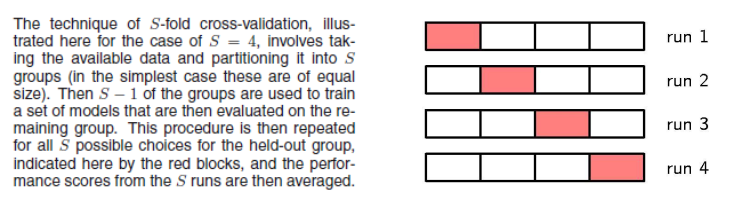
\includegraphics[width=100mm]{CrossValidation}

split training data into \textbf{training set} and \textbf{validation set}. Train different
models on training set and choose model with minimum error on validation set.
\subsection{decision theory}
\label{sec:org91d5478}
Suppose we have an input vector \(\bl{x}\) together with a corresponding vector
\(\bl{t}\) of target variables and our goal is to predict \(\bl{t}\) given new
value for \(\bl{x}\). The joint probability distribution \(p(\bl{x},\bl{t})\)
provides a complete summary of the uncertainty with these variables
\section{Statistical learning and modeling - Supervised learning}
\label{sec:org56eea98}
\subsection{Basic concepts}
\label{sec:org938d97f}
\begin{itemize}
\item \textbf{Linearly separable}
\begin{itemize}
\item decision regions:

input space is divided into several regions
\item decision boundaries:
\begin{itemize}
\item under linear models, it's a linear function
\item (D-1)-dimensional hyper-plane within the D-dimensional input space
\end{itemize}
\end{itemize}
\item \textbf{representation of class labels}
\begin{itemize}
\item Two classes K = 2
\item K classes
\begin{itemize}
\item 1-of-K coding scheme \(\bl{t}=(0,0,1,0,0)^T\)
\end{itemize}
\item Predict discrete class labels
\begin{itemize}
\item linear model prediction \(y(\bl{x})=\bl{w}^T\bl{x}+w_0\)
w: weight vector, w\textsubscript{0} bias/threshold
\item nonlinear function \(f(.):R\to(0,1)\)
\item generalized linear models
\(y(\bl{x})=f(\bl{w}^T\bl{x}+w_0)\)
f:activation function
\item dicision surface
\(y(\bl{x})=\text{constant}\to \bl{w}^T\bl{x}+w_0=\text{constant}\)
\end{itemize}
\end{itemize}
\item \textbf{Three classification approaches}
\begin{itemize}
\item discriminant function
\begin{itemize}
\item least squares approach
\item fisher's linear discriminant
\item the perceptron algorithm of rosenblatt
\end{itemize}
\item use discriminant functions directly and don't compute probabilities

Given discriminant functions \(f_1(\bl{x}),\dots,f_K(\bl{x})\). Classify
\(\bl{x}\) as class \(\mathcal{C}_k\) iff \(f_k(\bl{x})>f_j(\bl{x}),\forall
       j\neq k\)

\begin{itemize}
\item \textbf{least-squares approach}: making the model predictions as close as
possible to a set of target values
\item \textbf{fisher's linear discriminant}: maximum class separation in the ouput
space
\item \textbf{the perceptron algorithm of rosenblatt}
\end{itemize}
\item generative approach
\begin{itemize}
\item model the class-conditional densities and the class priors
\item compute posterior probabilities through Bayes's theorem

\(\underbrace{p(\mathcal{C}_k|\bl{x})}_\text{posterior for class}=
         \frac{\overbrace{p(\bl{x}|\mathcal{C}_k)}^\text{class conditional density}
         \overbrace{p(\mathcal{C}_k)}^\text{class prior}}{p(\bl{x})}=
         \frac{p(\bl{x}|\mathcal{C}_k)p(\mathcal{C}_k)}{\sum_{j}p(\bl{x}|\mathcal{C}_j)
         p(\mathcal{C}_j)}\)
\end{itemize}
\end{itemize}
\end{itemize}
\subsection{discriminant functions}
\label{sec:orge8b8a8d}
\subsubsection{Two classes}
\label{sec:orgb3068f5}
\begin{itemize}
\item Linear discriminant function \(y(\bl{x})=\bl{w}^T\bl{x}+w_0\)
\begin{itemize}
\item Dicision surface \(\Omega:y(\bl{x})=0\)
\item the normal distant from the origin to the dicision surface
\(\frac{\bl{w}^T\bl{x}}{\norm{\bl{w}}}=-\frac{w_0}{\norm{\bl{w}}}\)
\item if \(x_A,x_B\) lie on the decision surface \(y(\bl{x}_A)=y(\bl{x}_B)=0\),
then \(\bl{w}^T(\bl{x}_A-\bl{x}_B)=0\). hence w is orthogonal to every
vector lying within Ω. \(\frac{\bl{w}}{\norm{\bl{w}}}\) is the normal
vector of Ω

\item \(\bl{x}=\bl{x}_\perp+r\frac{\bl{w}}{\norm{\bl{w}}}\) hence
\(r=\frac{y(\bl{x})}{\norm{\bl{w}}}\). \(y(\bl{x}_\perp)=0\to
        \bl{w}^T\bl{x}=-w_0+r\frac{\bl{w}^T\bl{w}}{\norm{\bl{w}}}\)
\item \(\tilde{\bl{w}}=(w_0,\bl{w}), \tilde{\bl{x}}=(x_0,\bl{x}),
        y(\bl{x})=\tilde{\bl{w}}^T\tilde{\bl{x}}\)
\end{itemize}
\end{itemize}
\subsubsection{K-class}
\label{sec:orgee14ff6}
\begin{itemize}
\item One-versus-the-rest classifier
K - 1 classifiers each of which solves a two-class problem
\item One-versus-one classifier
K(K-1)/2 binary discriminant functions
\item single K-class discriminant comprising K linear functions
\(y_k(\bl{x})=\bl{w}_k^T\bl{x}+w_{k_0}\)
\begin{itemize}
\item assigning a point x to class \(\mathcal{C}_k\) if
\(y_k(\bl{x}>y_j(\bl{x}))\) for all j≠k
\item dicision boundary between class \(\mathcal{C}_k, \mathcal{C}_j\) is given
\(y_k(\bl{x})=y_j(\bl{x})\to
        (\bl{w}_k-\bl{w}_j)^T\bl{x}+(w_{k_0}-w_{j_0})=0\)
\item \(\mathcal{R}_k\) is singly connected convex
\item \(\hat{\bl{x}}=\lambda\bl{x}_A+(1-\lambda)\bl{x}_B\) where \(0\le\lambda\le
        1\), \(y_k(\hat{\bl{x}})=\lambda y_k(\bl{x}_A)+(1-\lambda)y_k(\bl{x}_B)\)
and hence \(\hat{x}\) also lies inside \(\mathcal{R}_k\)
\end{itemize}
\end{itemize}
\subsubsection{Learning the parameters of linear discriminant functions}
\label{sec:orgb625ceb}
\begin{enumerate}
\item Linear basis function models
\label{sec:org46dc0f8}
\textbf{linear regression}:
\(y(\bl{x},\bl{w})=w_0+w_1x_1+\dots+w_Dx_D=\bl{w}^T\bl{x}\).

For nonlinear functions \(\phi_j\),
\(y(\bl{x},\bl{w})=w_0+\displaystyle\sum_{j=1}^{M-1}
     w_j\phi_j(\bl{x})=\bl{w}^T\bl{\phi(\bl{x})}\) where \(\phi_j(\bl{x})\) are
\textbf{basis functions} 
\item \textbf{parameter optimization via maximum likelihood}
\label{sec:orgc9d9d7d}

Assume target variable \(t\) is given by a deterministic function
\(y(\bl{x},\bl{w})\) with additive Gaussian noice so that
\(t=y(\bl{x},\bl{w})+\epsilon\) where \(\epsilon\) is a zero mean Gaussian
random variable with precision \(\beta\), hence we can write
\begin{equation*}
p(t|\bl{x},\bl{w},\beta)=\mathcal{N}(t|y(\bl{x},\bl{w}),\beta^{-1})
\end{equation*}
and \(\mathbb{E}(t|\bl{x})=\int tp(t|\bl{x})dt=y(\bl{x},\bl{w})\)

For data set \(\bl{X}=\{\bl{x}_1,\dots,\bl{x}_n\},\bl{t}=(t_1,\dots,t_n)^T\),
\(p(\bl{t}|\bl{X},\bl{w},\beta)=\displaystyle\prod_{n=1}^N\mathcal{N}(t_n|
     \bl{w}^T\bl{\phi}(\bl{x}_n),\beta^{-1})\)

\(\ln p(\bl{t}|\bl{w},\beta)=\displaystyle\sum_{n=1}^N\ln\mathcal{N}(t_n|
     \bl{w}^T\bl{\phi}(\bl{x}_n),\beta^{-1})=\frac{N}{2}\ln\beta-\frac{N}{2}\ln(2\pi)-
     \beta E_D(\bl{w})\)

\(E_D(\bl{w})=\frac{1}{2}\displaystyle\sum_{n=1}^N
     \left\{t_n-\bl{w}^T\bl{\phi}(\bl{x}_n)\right\}^2=
     \frac{1}{2}\norm{t-\Phi\bl{w}}\) is sum-of-squares error function

solve \(\bl{w}\) by maximum likelihood.
\begin{equation*}
\nabla\ln p(\bl{t}|\bl{w},\beta)=\displaystyle\sum_{n=1}^N
\left\{t_n-\bl{w}^T\bl{\phi}(\bl{x}_n)\right\}\phi(\bl{x}_n)^T
\end{equation*}
\begin{equation*}
0=\displaystyle\sum_{n=1}^N t_n\bl{\phi}(\bl{x}_n)^T-\bl{w}^T
(\displaystyle\sum_{n=1}^N\bl{\phi}(\bl{x}_n)\bl{\phi}(\bl{x}_n)^T)
\end{equation*}
Hence we get
\begin{equation*}
\bl{w}_{ML}=(\bl{\Phi}^T\bl{\Phi})^{-1}\bl{\Phi}^T\bl{t}
\end{equation*}
\(\Phi\) is \textbf{design matrix}.
\[
\Phi=\begin{pmatrix}
 \phi_0(\bl{x}_1) & \phi_1(\bl{x}_1) & \dots & \phi_{M-1}(\bl{x}_1) \\
 \phi_0(\bl{x}_2) & \phi_1(\bl{x}_2) & \dots & \phi_{M-1}(\bl{x}_2) \\
 \vdots & \vdots & \ddots & \vdots \\
 \phi_0(\bl{x}_N) & \phi_1(\bl{x}_N) & \dots & \phi_{M-1}(\bl{x}_N) \\
\end{pmatrix}
\]

For bias parameter \(w_0\).
\(E_D(\bl{w})=\frac{1}{2}\displaystyle\sum_{n=1}^N 
     \{t_n-w_0-\displaystyle\sum_{j=1}^{M-1}w_j\phi_j(\bl{x}_n)\}^2\). Hence
\(w_0=\bar{t}-\displaystyle\sum_{j=1}^{M-1}w_j\bar{\phi_j}\),
\(\bar{t}=\frac{1}{N}\displaystyle\sum_{n=1}^Nt_n\),
\(\bar{\phi_j}=\frac{1}{N}\displaystyle\sum_{n=1}^N\phi_j(\bl{x}_n)\).

\(frac{N}{2\beta}=E_D(\bl{w})\). \(\frac{1}{\beta_{ML}}=
     \frac{1}{N}\displaystyle\sum_{n=1}^N\left\{t_n-\bl{w}^T_{ML}
     \bl{\phi}(\bl{x}_n)\right\}^2\)
\item Least-squares approach
\label{sec:orge3fd5c9}
\begin{itemize}
\item Problem
\begin{itemize}
\item Each class \(\mathcal{C}_k\) is described by its own linear model 
\(y_k(\bl{x})=\bl{w}_k^T\bl{x}+w_{k0}\)
\item group together: \(y(\bl{x})=\widetilde{\bl{W}}^T\tilde{\bl{x}}\),
\(\tilde{\bl{w}}_k=(w_{k0},\bl{w}_k^T)^T\), \(\tilde{\bl{x}}=(1,\bl{x}^T)^T\)
\end{itemize}
\item Learning
\begin{itemize}
\item minimizing SSE function sum-of-squares
\(SSE=\displaystyle\sum_{i=1}^n(y_i-f(x_i))^2\)
\(E_D(\widetilde{\bl{W}})=1/2\text{Tr}\{(\bl{\widetilde{X}\widetilde{W}-T})^T 
         (\bl{\widetilde{X}\widetilde{W}-T})\}\)

\(\bl{\widetilde{W}}=(\bl{\widetilde{X}}^T\bl{\widetilde{X}})^{-1}\bl{\widetilde{X}}^T\bl{T}\)
\end{itemize}
\end{itemize}
\item fisher's linear discriminant
\label{sec:org21d31a0}

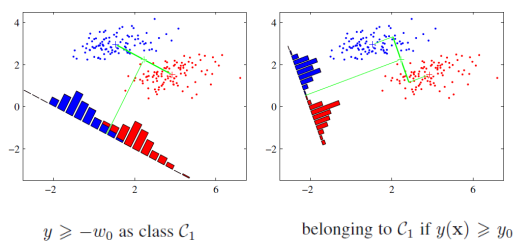
\includegraphics[width=100mm]{Fisher}

from the view of dimensionality reduction
\(y\ge -w_0\) as class \(\mathcal{C}_1\)

\(m_1=\frac{1}{N_1}\displaystyle\sum_{n\in\mathcal{C}_1}x_n, 
     m_2=\frac{1}{N_2}\displaystyle\sum_{n\in\mathcal{C}_2}x_n
     \xrightarrow{y=\bl{w}^T\bl{x}} m_2-m_1=\bl{w}^T(\bl{m}_2-\bl{m}_1)\)
\item the perceptron algorithm of rosenblatt
\label{sec:org1ca60b4}
\end{enumerate}
\subsection{probalibilistic generative models}
\label{sec:orgd7e1496}
A probabilistic view of classification from simple assumptions about the
distribution of the data

\begin{align*}
p(\mathcal{C}_1|\bl{x})&=\frac{p(\bl{x}|\mathcal{C}_1)p(\mathcal{C}_1)}
{p(\bl{x}|\mathcal{C}_1)p(\mathcal{C}_1)+p(\bl{x}|\mathcal{C}_2)p(\mathcal{C}_2)}\\
&=\frac{1}{1+\exp(-a)}=\sigma(a)
\end{align*}
where 
\begin{equation*}
a=\ln\frac{p(\bl{x}|\mathcal{C}_1)p(\mathcal{C}_1)}
{p(\bl{x}|\mathcal{C}_2)p(\mathcal{C}_2)}
\end{equation*}
and \(\sigma(a)\) is the \textbf{logistic sigmoid} function defined by
\begin{equation*}
\sigma(a)=\frac{1}{1+\exp(-a)}
\end{equation*}
and \(\sigma(-a)=1-\sigma(a)\), its inverse is \textbf{logit} function
\begin{equation*}
a=\ln(\frac{\sigma}{1-\sigma})
\end{equation*}

For case of \(K > 2\) classes, we have the following \textbf{multi-class generalization}
\begin{equation*}
p(\mathcal{C}_k|\bl{x})=\frac{p(\bl{x}|\mathcal{C}_k)p(\mathcal{C}_k)}
{\sum_jp(\bl{x}|\mathcal{C}_j)p(\mathcal{C}_j)}=\frac{\exp(a_k)}{\sum_j\exp(a_j)},
a_k=\ln\left[p(\bl{x}|\mathcal{C}_k)p(\mathcal{C}_k)\right]
\end{equation*}
The \textbf{normalized exponential} is known as the \textbf{softmax function} as it represents
a \emph{smoothed version of the max function}
\begin{equation*}
\text{if } a_k\ll a_j,\forall j\neq k,\text{then } p(\mathcal{C}_k|\bl{x})\approx 1,
p(\mathcal{C}_j|\bl{x})\approx 0
\end{equation*}

For \textbf{continuous inputs}, assume
\begin{equation*}
p(\bl{x}|\mathcal{C}_k)=\frac{1}{(2\pi)^{D/2}}\frac{1}
{\abs{\bl{\Sigma}}^{1/2}}\exp\left\{-\frac{1}{2}(\bl{x}-\bl{\mu}_k)^T
\bl{\Sigma^{-1}}(\bl{x}-\bl{\mu}_k)\right\}
\end{equation*}
\begin{enumerate}
\item 2 classes
\begin{align*}
p(\mathcal{C}_1|\bl{x})&=\sigma(\bl{w}^T\bl{x}+w_0)\\
\bl{w}&=\bl{\Sigma}^{-1}(\bl{\mu}_1-\bl{\mu}_2)\\
w_0&=-\frac{1}{2}\bl{\mu}_1^T\bl{\Sigma}^{-1}\bl{\mu}_1+
\frac{1}{2}\bl{\mu}_2^T\bl{\Sigma}^{-1}\bl{\mu}_2+\ln\frac{p(\mathcal{C}_1)}
{p(\mathcal{C}_2)}\\
\end{align*}
\item K classes
\begin{align*}
a_k(\bl{x})&=\bl{w}_k^T\bl{x}+w_{k0}\\
\bl{w}_k&=\bl{\Sigma}^{-1}\bl{\mu}_k\\
w_{k0}&=-\frac{1}{2}\bl{\mu}_k^T\bl{\Sigma}^{-1}\bl{\mu}_k+\ln p(\mathcal{C}_k)
\end{align*}
\end{enumerate}
\subsection{probabilistic discriminative models}
\label{sec:org858e325}
\subsection{Boosting}
\label{sec:orgdba8fbe}
Originally designed for classification problems.

Motivation: a procedure that combines the outputs of many "weak" classifiers
to produce a strong/accurate classifier


\subsubsection{AdaBoost}
\label{sec:org9625e9f}
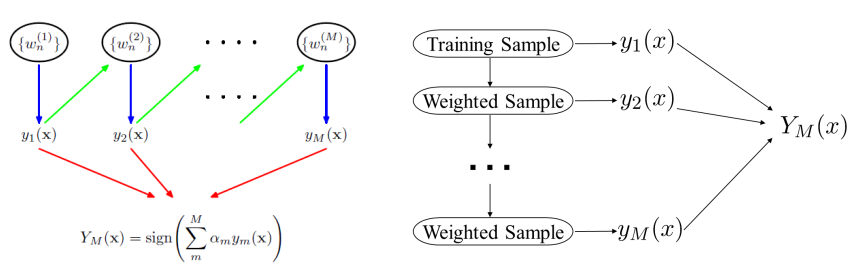
\includegraphics[width=100mm]{Boosting}
\section{unsupervised learning - clustering em and PCA}
\label{sec:org9561bab}
\subsection{K-means clustering}
\label{sec:org1cb8443}
\begin{itemize}
\item Distortion measure
\(J=\displaystyle\sum_{n=1}^N \displaystyle\sum_{k=1}^Kr_{nk}
     \norm{\bl{x}_n-\bl{\mu}_k}^2\)
\end{itemize}
\subsection{Mixtures of Gaussians}
\label{sec:org3ecfc9b}
\begin{itemize}
\item Definition: 
\begin{equation*}
p(\bl{x})=\displaystyle\sum_{k=1}^K\pi_k\mathcal{N}
(\bl{x}|\bl{\mu}_k,\bl{\Sigma}_k)\quad \displaystyle\sum_{k=1}^k\pi_k=1
\quad 0\le\pi_k\le1
\end{equation*}
\item introduce a K-dimensional binary random variable \(\bl{z}=(z_1,\dots,z_k)^T\)
\begin{equation*}
z_k\in\{0,1\}\quad \displaystyle\sum_kz_k=1\quad p(z_k=1)=\pi_k
\end{equation*}

Hence \(p(\bl{z})
     =\displaystyle\prod_{k=1}^K\pi_k^{z_k}\), \(\bz\) is \textbf{latent variable} (inferred
from other observed variables)

If \(p(\bl{x}|z_k=1)=\mathcal{N}(\bl{x}|\bl{\mu}_k,\bl{\Sigma})\), then
\(p(\bl{x}|\bl{z})=\displaystyle\prod_{k=1}^K\mathcal{N}(\bl{x}|\bl{\mu}_k,
     \bl{\Sigma}_k)^{z_k}\)
\item \textbf{equivalent formulation} of the Gaussian mixture.
\begin{align*}
\Aboxed{
p(\bl{x})&=\displaystyle\sum_{\bl{z}}p(\bl{x}|\bl{z})p(\bl{z})
=\displaystyle\sum_{\bl{z}}\displaystyle\prod_{k=1}^K
\mathcal{N}(\bl{x}|\bl{\mu}_k,\bl{\Sigma}_k)^{z_k}}\\
&=\displaystyle\sum_{j=1}^K\displaystyle\prod_{k=1}^K\mathcal{N}(\bl{x}|\bl{\mu}_k,
\bl{\Sigma}_k)^{I_{kj}}\quad I_{kj}=
\begin{cases}
1&\text{if } k=j\\
0&\text{otherwise}
\end{cases}\\
&=\displaystyle\sum_{j=1}^K\pi_j\mathcal{N}(\bl{x}|\bl{\mu}_j,\bl{\Sigma}_j)
\end{align*}

responsibility:
\begin{equation*}
\gamma(z_k)=p(z_k=1|\bx)=\frac{p(z_k=1)p(\bx|z_k=1)}{\dissum_{j=1}^Kp(z_j=1)p(\bx|z_j=1)}
=\frac{ \pi_k\caln(\bx|\bmu_k,\bSigma)}{\dissum_{j=1}^K\pi_j\caln(\bx|\bmu_j
\bSigma_j)}
\end{equation*}
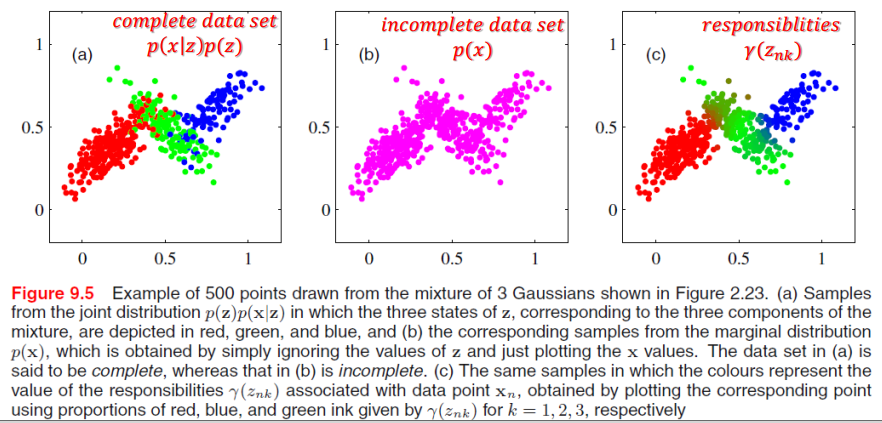
\includegraphics[width=130mm]{GMM}
\end{itemize}

\textbf{Expectation-Maximization algorithm for GMM}. 
\(p(\bX|)=\dispro p(\bx)\)

\(\ln p(\bX|\pi,\bmu, \bSigma)=\dissum_{n=1}^N\ln\left\{
   \dissum_{k=1}^K\pi_k\caln(\bx_n|\bmu_k,\bSigma_k)\right\}\)
\begin{enumerate}
\item E step
\begin{equation*}
\gamma(z_{nk})=\frac{\pi_k\caln(\bx_n|\bmu_k,\bSigma_k)}
{\dissum_j\pi_j\caln(\bx_n|\bmu_j,\bSigma_j)}
\end{equation*}
\item M step
\begin{itemize}
\item solve \(\bmu_k\)
\begin{align*}
&\frac{\partial\ln p(\bX|\pi,\bmu,\bSigma)}{\partial\bmu_k}=0\\
&0=-\frac{\pi_k\caln(\bx_n|\bmu_k,\bSigma_k)}
{\dissum_j\pi_j\caln(\bx_n|\bmu_j,\bSigma_j)}\bSigma_k^{-1}(\bx_n-\bmu_k)\\
&\bmu_k=\frac{1}{N_k}\dissum_{n=1}^N\gamma(z_{nk})\bx_n\\
&N_k=\dissum_{n=1}^N\gamma(z_{nk})
\end{align*}
\item solve \(\bSigma_k\)
\begin{align*}
&\frac{\partial\ln p(\bX|\pi,\bmu,\bSigma)}{\partial\bSigma_k}=0\\
&\bSigma_k=\frac{1}{N_k}\dissum_{n=1}^N\gamma(z_{nk})(\bx_n-\bmu_k)(\bx_n-\bmu_k)^T
\end{align*}
\end{itemize}
\end{enumerate}


\textbf{EM for Gaussian Mixtures}
\begin{enumerate}
\item initialize the means \(\bmu_k\), covariances \(\bSigma_k\) and mixing
coefficients \(\pi_k\)
\item E step
\item M step
\item evaluate the log likelihood
\begin{equation*}
\ln p(\bX|\pi,\bmu, \bSigma)=\dissum_{n=1}^N\ln\left\{
\dissum_{k=1}^K\pi_k\caln(\bx_n|\bmu_k,\bSigma_k)\right\}
\end{equation*}
and check for convergence of either the parameters or the log likelihood.
If the convergence criterion is not satisfied return to step 2
\end{enumerate}
\subsection{An alternative view of EM}
\label{sec:orgf62dca0}
\subsubsection{the general EM algorithm}
\label{sec:org138aeb4}
The log likelihood of a discrete latent variables model
\begin{equation*}
\ln p(\bX|\theta)=\ln\lb\dissum_{\bZ} p(\bX,\bZ|\btheta)\rb
\end{equation*}


\emph{the goal of EM algorithm is to find maximum likelihood solution for models
having latent variables} 


For the complete data set \(\lb\bX,\bZ\rb\), the likelihood function
\begin{equation*}
\ln p(\bX|\btheta)\Longrightarrow \ln p(\bX,\bZ|\btheta)
\end{equation*}


For the incomplete data set \(\lb\bX\rb\), we adopt the following steps to
find maximum likelihood solution
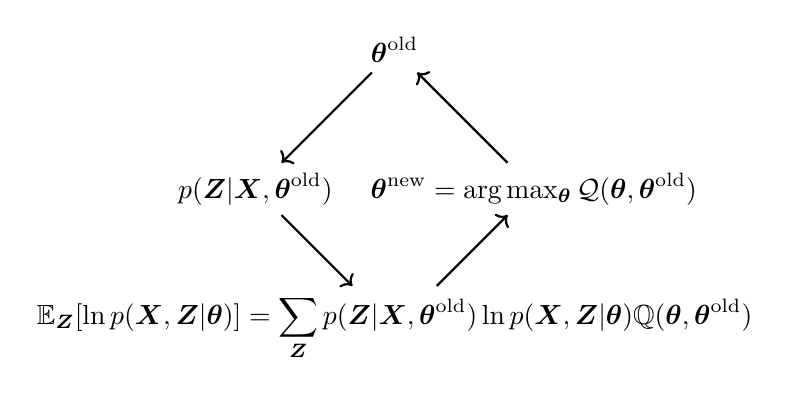
\begin{tikzpicture}[node distance=2.5cm]
\tikzstyle{arrow}=[->,thick];
\node (1) [] {$\btheta^\text{old}$};
\node (2) [below left of=1] {$p(\bZ|\bX,\btheta^\text{old})$};
\node (3) [below right of=2] {$\E_{\bZ}[\ln p(\bX,\bZ|\btheta)]=\displaystyle\sum_{\bZ}
p(\bZ|\bX,\btheta^\text{old})\ln p(\bX,\bZ|\btheta)\Q (\btheta,\btheta^\text{old})$};
\node (4) [below right of=1] {$\btheta^\text{new}=\text{arg} \max_{\btheta}\calq(\btheta,\btheta^\text{old})$};
\draw [arrow] (1) -- (2);
\draw [arrow] (2) -- (3);
\draw [arrow] (3) -- (4);
\draw [arrow] (4) -- (1);
\end{tikzpicture}
\section{reinforcement learning}
\label{sec:org052f646}

\section{wef}
\label{sec:org9d6a7c5}
\subsection{wfe}
\label{sec:orgf6341a5}
K-means
\end{document}